\documentclass[a4paper, 11pt]{article}
\usepackage{covington}
\usepackage{amssymb}
\usepackage{amsmath}
\usepackage[catalan]{babel}
\usepackage{graphicx}
\usepackage{eurosym}
\textheight=23.94cm 
\textwidth=17cm 
\topmargin=-1cm 
\oddsidemargin=-0.5cm 
 
\newcommand{\header}[4]{
	\begin{center}
		\rule{\linewidth}{0.5pt}
		
		{\small{#1}}
      
        \vspace{0.2in}
        
		{\large{#2}}
		
        \vspace{0.2in}
        
		{\small{#3}}
		
		\vspace{0.15in}
		
		{#4}
		
		\vspace{-0.1in}
		\rule{\linewidth}{0.6pt}
	\end{center}
}

\begin{document}
 
\header{\sc Barcelona Graduate School of Economics \hfill Master's Degree in Data Science}{\bf Statistical Modeling and Inference $-$ Problem Set \#3}{\sc Niti Mishra $\cdot$ Miquel Torrens $\cdot$ B\'alint V\'an}{October 26\textsuperscript{th}, 2015}
Solution to proposed exercises.\\
% EXERCISE 1
\newline \textbf{\underline{Exercise 1}}\\
\newline The exercise requires two extra parameters not defined, which are $\delta$ and $g$.\\
\newline We keep $\delta$ as the degree of freedom. We will try to find $g$ in the following manner:
\begin{itemize}
\item To start, we compute the sample variance of the model with only the intercept.
\item We plug the result in out first Bayesian iteration as a proxy for $g$, given a $\delta$.
\item We obtain an updated result on $g$ after running the model and we use this result to re-run the model for a new $g$.
\item We keep running models until we detect that $g$ stabilizes and we keep that stable $g$ for the ultimate model.
\end{itemize}
The model shall look as follows:\\
\begin{center}
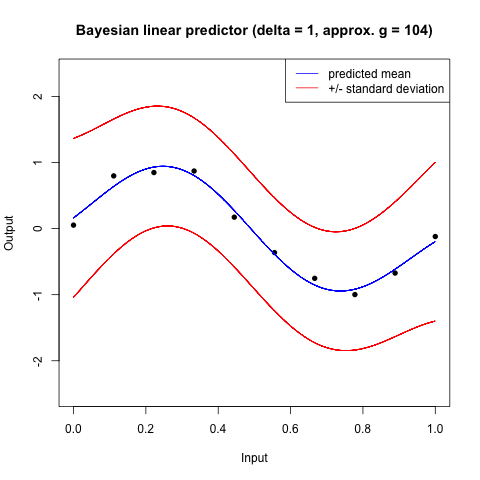
\includegraphics[scale=0.6]{ps3F_plot1.png}
\end{center}
We will plot the results of posterior draws using $\delta=2$, as used in previous exercises, since it is the value that best suits these data (see lectures).
\begin{center}
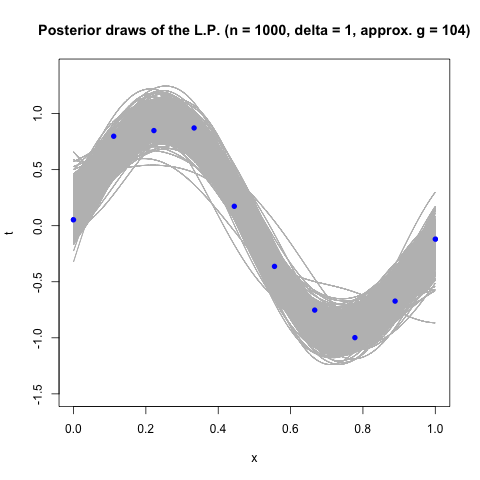
\includegraphics[scale=0.6]{ps3F_plot2.png}
\end{center}
Now we explore how the models are sensible to $\delta$. Note that we fix the value of $\delta$ and that $g$ is then determined by the aforementioned algorithm:\\
\begin{center}
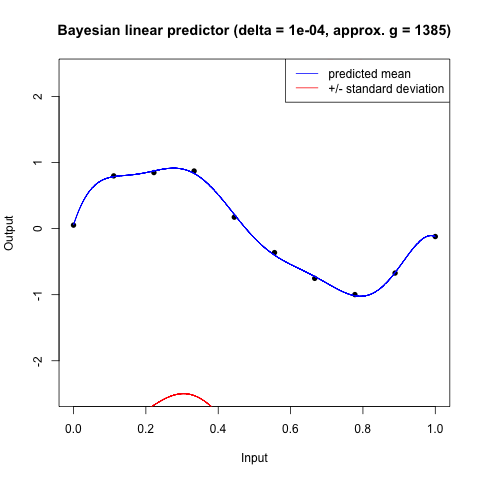
\includegraphics[scale=0.6]{ps3F_plot3_1.png}
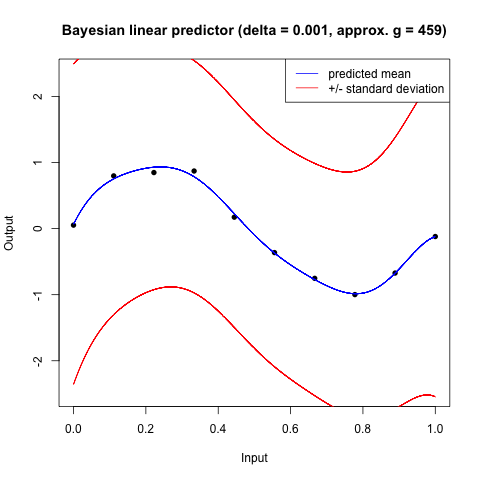
\includegraphics[scale=0.6]{ps3F_plot3_2.png}
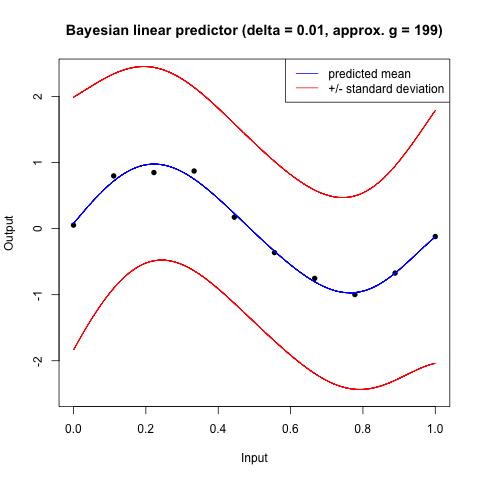
\includegraphics[scale=0.6]{ps3F_plot3_3.png}
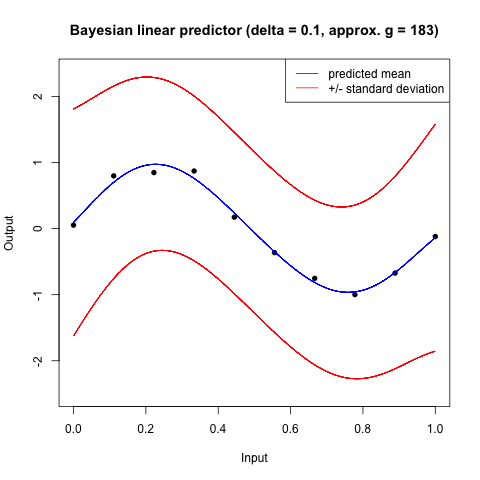
\includegraphics[scale=0.6]{ps3F_plot3_4.png}
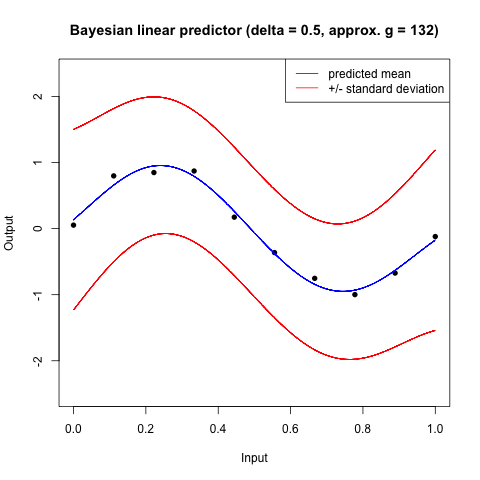
\includegraphics[scale=0.6]{ps3F_plot3.png}
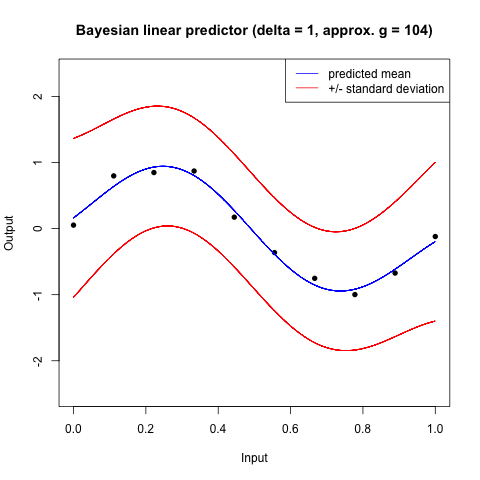
\includegraphics[scale=0.6]{ps3F_plot4.png}
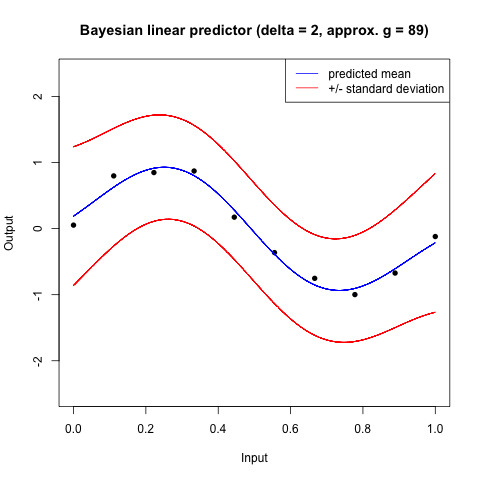
\includegraphics[scale=0.6]{ps3F_plot5.png}
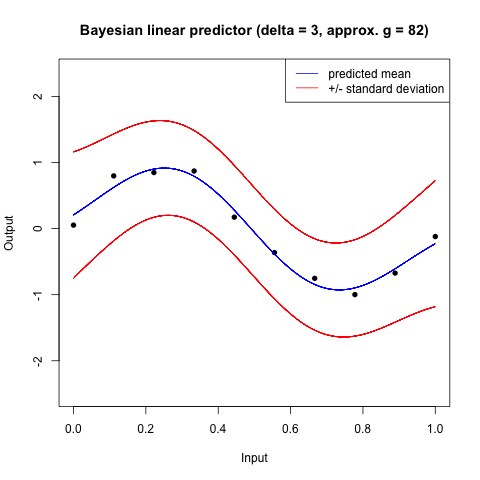
\includegraphics[scale=0.6]{ps3F_plot6.png}
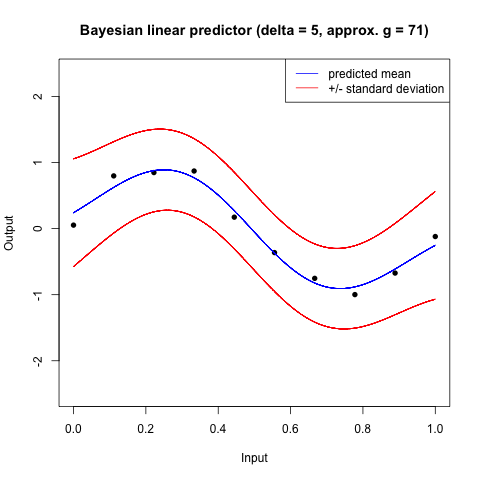
\includegraphics[scale=0.6]{ps3F_plot7.png}
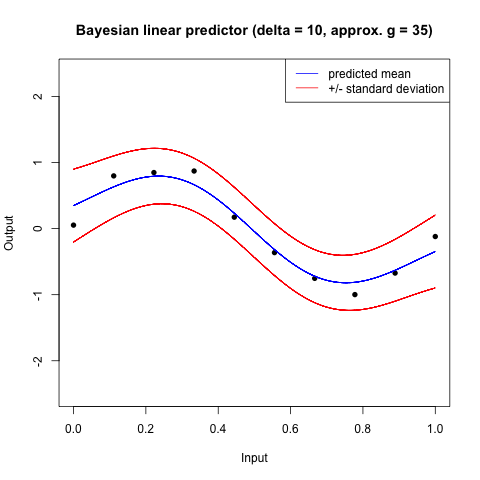
\includegraphics[scale=0.6]{ps3F_plot8.png}
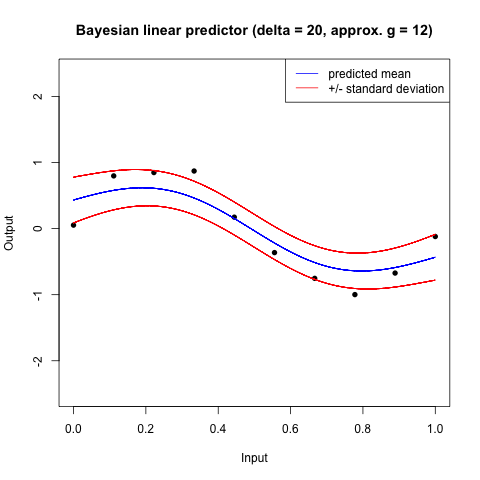
\includegraphics[scale=0.6]{ps3F_plot9.png}
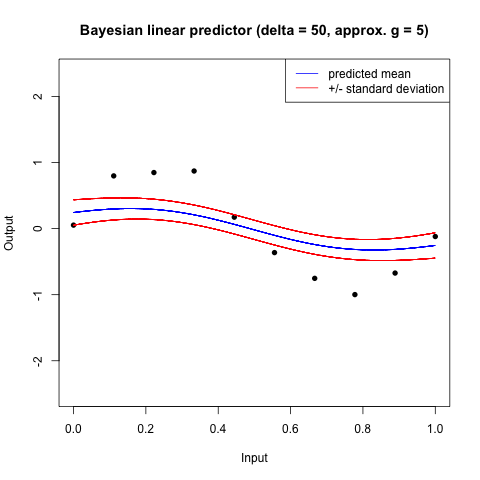
\includegraphics[scale=0.6]{ps3F_plot10.png}
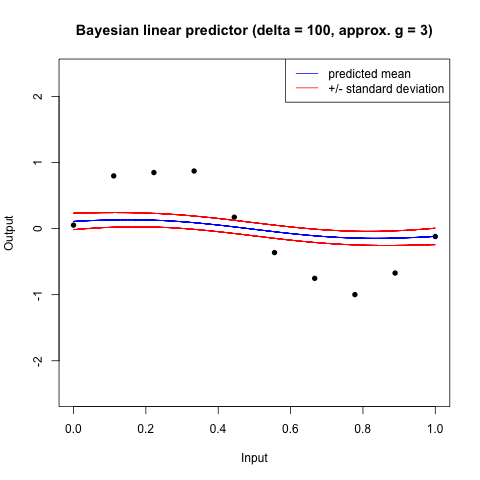
\includegraphics[scale=0.6]{ps3F_plot11.png}
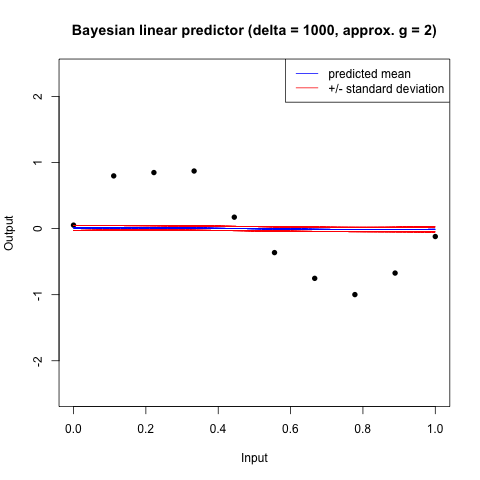
\includegraphics[scale=0.6]{ps3F_plot12.png}
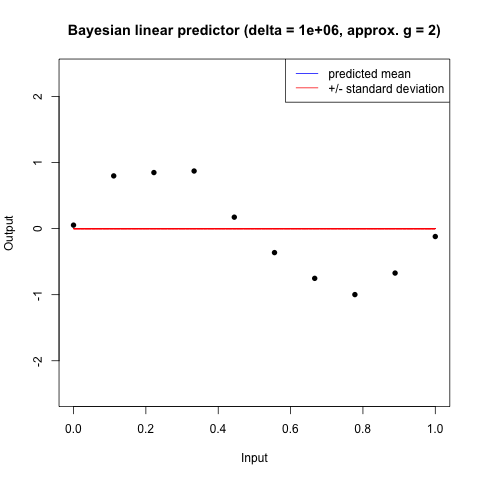
\includegraphics[scale=0.6]{ps3F_plot13.png}
\end{center}
Note that as $\delta$ increases (and $g$ decreases), the prediction becomes flatter and errors become bigger, with a .\\
% EXERCISE 2
\newline \textbf{\underline{Exercise 2}}\\

\end{document}